
\begin{figure}[h]
\centering \sffamily

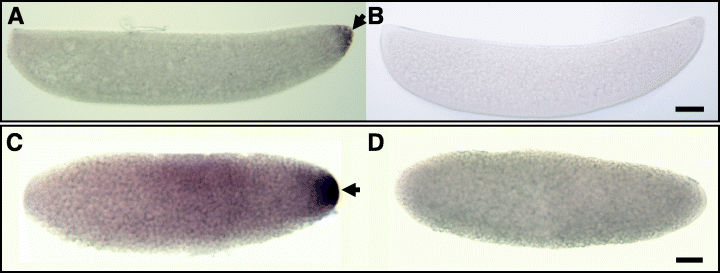
\includegraphics[width=.8\textwidth]{figures/figs/oskar_expression_AaAg.png}

\caption[\textit{oskar} gene expression in the vector mosquitoes, \Ang\ and \Aea]{\sf \textbf{\textit{oskar} gene expression in the vector mosquitoes, \Ang\ and \Aea:} \\
 Hybridizations \textit{in situ} of \textit{Anga osk} and \textit{Aeae osk} RNA probes to whole-mount \Ag\ and \Aa\ embryos. Embryos are orientated with anterior on the left. \Ag\ embryos (A,B) shown have reached cellular blastoderm with pole cells indicated by an arrow. \Aa\ embryos (C,D) shown are in the preblastoderm stage. Strong staining is exclusive to the posterior pole cells (A) and posterior end (C) (arrows), when compared with embryos of the same stage, determined by DAPI staining (not shown), probed with \textit{Anga} and \textit{Aeae osk} sense RNA probes (B,D). Bar = 50 µm.\\
 
 Excerpted from \cite{Juhn2006}}\label{fig:pole-cells}
\end{figure}